\documentclass[12pt]{article}
\usepackage[a4paper,margin=1in,footskip=0.25in]{geometry} % set margins
\usepackage[portuguese]{babel}
\usepackage[utf8]{inputenc}
\usepackage{hyperref} 
\usepackage{amsmath}
\usepackage{amssymb}
\usepackage{amsthm}
\usepackage{graphicx} % include graphics
\usepackage{indentfirst}
\usepackage{float} % used for [H] figure option


% Macros
\newcommand{\questao}[1] {\vspace{12pt} \noindent \large \textbf{Questão #1:} \normalsize}
\renewcommand{\part}[1] {\noindent\textbf (#1)}
\renewcommand{\familydefault}{\sfdefault} % sans-serif


\begin{document}
\title{EP1 - MAC0210}
\begin{flushleft}
    \textbf{\fontsize{20pt}{2em}\selectfont 
        MAC0210 - Exercício Programa 1\\}
    \fontsize{10pt}{1em}\selectfont{Professor: 
        \href{mailto:egbirgin@gmail.com}{Ernesto G. Birgin}\\
    Monitor: 
        \href{mailto:estrela.gustavo.matos@gmail.com}{Gustavo Estrela}\\}
\end{flushleft}


\section {Parte 1: Aritmética de Ponto Flutuante}
    Essa parte do EP consiste em resolver quatro exercícios sobre 
aritmética de ponto flutuante. Para solucionar os problemas é
recomendado a leitura do livro "Numerical Computing with IEEE Floating
Point Arithmetic", presente na 
\href{http://ime.usp.br/~egbirgin/mac210/biblio.html}{bibliografia} do 
curso. Todos os exercícios da parte 1 desse EP foram inspirados em 
exercícios do livro, indicados entre parênteses.

    Você deve subir um arquivo pdf no paca com as suas soluções.
Além disso você deve entregar na aula do dia 20 de setembro uma 
cópia impressa do mesmo pdf que foi entregue no paca.

\questao{1 (3.11)} 
Suponha que temos um sistema de representação de ponto flutuante com
base 2 e,
\begin{center}
    \begin{tabular}{r l}
             & $x = \pm S \times 2^E$,\\ 
        com  & $S = (0.1b_2b_3b_4...b_{24})$, \\
        i.e, & $\frac{1}{2} < S < 1$
    \end{tabular}
\end{center}
onde o expoente $-128 < E < 127$. \\ 
\part{a} Qual é o maior número de ponto flutuante desse sistema? \\
\part{b} Qual é o menor número de ponto flutuante positivo desse 
sistema? \\
\part{c} Qual é o menor inteiro positivo que não é exatamente 
representável nesse sistema? \\

\questao{2 (5.1)}
Qual é a representação do número $1/10$ no formato IEEE single para
cada um dos quatro modos de arredondamento? E para os números 
$1 + 2^{-25}$ e $2^{130}$?\\

\questao{3 (6.4)}
Qual é o maior número de ponto flutuante $x$ tal que $1 \oplus x$ é
exatamente 1, assumindo que o formato usado é IEEE single e modo de 
arredondamento para o mais próximo? E se o formato for IEEE double?

\questao{4 (6.8)} Em aritmética exata, a soma é um operador
comutativo e associativo. O operador de soma de ponto flutuante é 
commutativo? E associativo? Explique.

\section{Parte 2: Método de Newton}
Quando se aplica o Método de Newton a uma função com mais de uma raíz,
temos que a raíz que será obtida pelo método depende do ponto inicial 
escolhido. Nesta parte do EP vamos extender o Método de Newton para um
domínio complexo e estudar suas \textbf{bacias de convergência}, o 
conjunto de pontos iniciais que convergem para uma mesma raíz da função
estudada.

Você deve implementar o Método de Newton em Octave e usar o script 
disponível em \href{algumlugar}{} para gerar uma imagem que mostra as
bacias de convergência de uma função escolhida. Você vai notar que as
imagens geradas formam fractais! Explicar o motivo da formação desses
fractais não é necessário. Veja abaixo alguns exemplos.

\begin{figure}[H]
    \begin{center}
        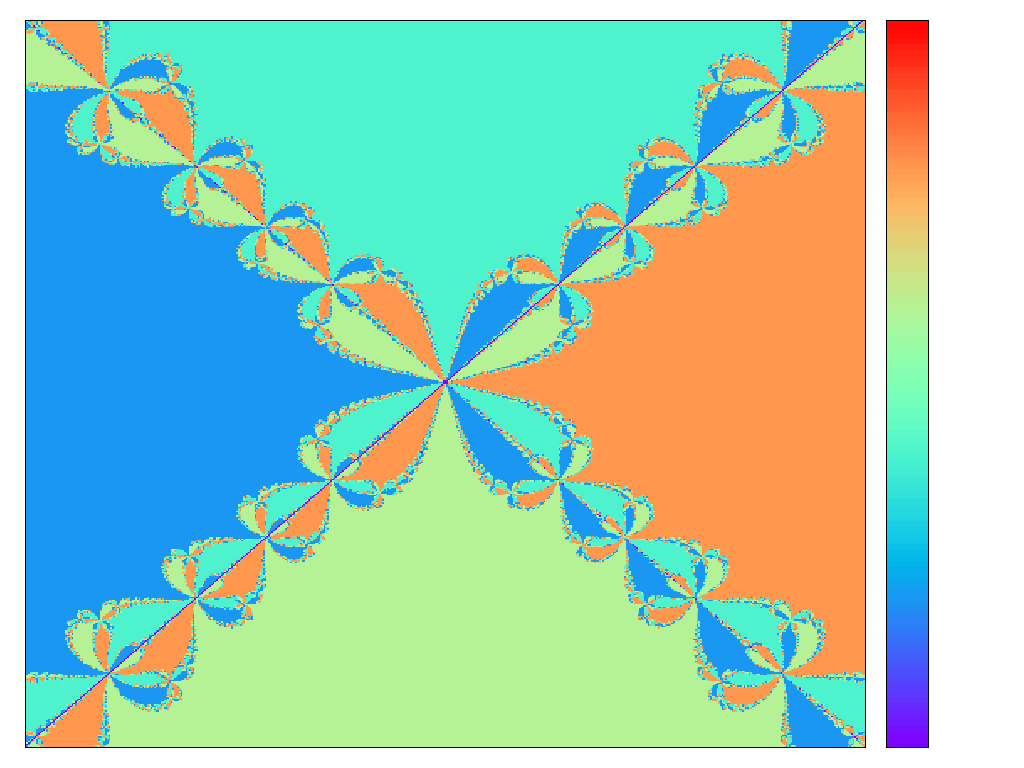
\includegraphics[scale = .4]{figures/x4-1}
    \end{center}
    \caption{Bacias de convergência do polinômio $x^4 - 1$. O plano
    visto varia de $-2$ a $2$ no eixo $x$ e de $-2i$ a $2i$ no eixo
    y}
    \label{fig:x4-1}
\end{figure}
\begin{figure}[H]
    \begin{center}
        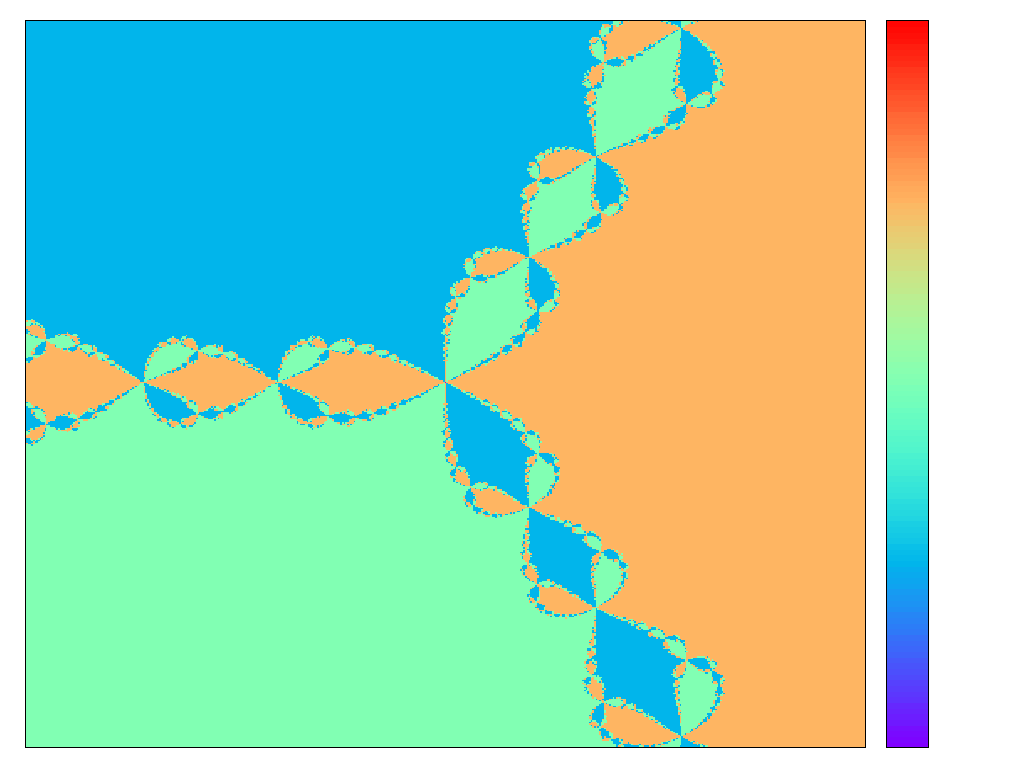
\includegraphics[scale = .4]{figures/x3-1}
    \end{center}
    \caption{Bacias de convergência do polinômio $x^3 - 1$. O plano
    visto varia de $-2$ a $2$ no eixo $x$ e de $-2i$ a $2i$ no eixo
    y}
\end{figure}

\subsection{Como gerar imagens das bacias de convergência}
O primeiro passo que você deve tomar para gerar as imagens é escolher
um subconjunto do plano complexo. Agora, associe a cada um dos $n^2$
($n$ é um parâmetro de sua função) pixels da imagem a um ponto do 
plano, rode o método de newton usando como início esse ponto e
descubra a raíz encontrada. Cada raíz do polinomio deve estar associada
a uma cor, que será pintada em todos os pontos iniciais que convergirem
para essa raíz.

As imagens das bacias de convergência devem ser geradas pelo programa
{\em gnuplot} usando o script disponibilizado, {\em plot\_basins}. Esse
script lê as linhas de um arquivo chamado {\em output.txt} que devem
conter uma tripla $x$ $y$ $r$ que representam respectivamente: a 
coordenada $x$ do pixel na \textbf{imagem gerada}; a coordenada $y$ do
pixel na \textbf{imagem gerada}; e um inteiro $r$ que representa a raíz
encontrada quando rodamos o Método de Newton usando o ponto associado a
$(x, y)$ como partida do algoritmo.

A escolha de criar um mapeamento entre as raízes de sua função para um
número inteiro $r$ se dá para facilitar a escolha de uma cor para cada
raíz. O script {\em plot\_basins} possui uma paleta de cores que
são usadas de acordo com o {\em range} definido no script em:
\begin{center}
    set cbrange [$a$ : $b$]
\end{center}
Na paleta usada na figura \ref{fig:x4-1}, por exemplo, uma raíz 
associada ao número $a$ teria cor roxa enquanto que uma raíz associada
ao número $b$ teria cor vermelha. Note que você também precisa associar
os pontos que não convergem a nenhuma raíz a uma cor. Você pode 
modificar o script que faz o plot ao seu gosto (sem mudar o formato dos
arquivos de entrada e saída) para criar imagens.


\subsection{Funções a serem implementadas}
Você deve implementar suas funções em um arquivo chamado 
{\em newton\_basins.m} que deve conter pelo menos as seguintes funções:
\begin{itemize}
    \item{newton\_basins ($f$, $n$):} acha as bacias de convergência da 
        função $f$ e gera um arquivo {\em output.txt} que contém os dados
        para geração da imagem das bacias pelo script {\em plot\_basins}.
        Os dados gerados preenchem uma imagem com $n \times n$ pixels.
    \item{newton ($f$, $f'$, $x_0$):} aplica o método de newton para 
        achar uma raíz da função $f$ (com primeira derivada $f'$), 
        partindo do ponto $x_0$.
\end{itemize}

\subsection{O que deve ser entregue}
Você deve entregar ao paca seu programa em Octave que implementa o 
Método de Newton como foi detalhado anteriormente e também um 
relatório sobre o problema em pdf. O relatório deve explicar como
você aplicou o Método de Newton e também deve conter exemplos 
interessantes com imagens geradas pelo seu programa (de preferência
diferentes das que foram apresentadas neste enunciado como exemplo).

\section{Parte 3 - Encontrando Todas as Raízes de Funções}
Escreva um programa em Octave para achar todas as raízes de uma função
$f \in C^2[a,b]$. Seu programa dividir $[a, b]$ em {\em ninter} 
sub-intervalos equidistantes e descobrir em quais deles a função f 
troca de sinal.

Para cada sub-intervalo $[a_i, b_i]$ sobre o qual $f(x)$ troca de
sinal, seu programa deve então achar as raízes da seguinte maneira. Use
o método de Newton ou secante para achar a raíz do intervalo, 
monitorando o decrescimento de $|f(x_k)|$. Se uma iteração é alcançada
tal que não há decrescimento suficiente de $|f(x_k)|$, i.e $|f(x_k)| > 
0.5 f(x_{k - 1})$, então volte ao intervalo $[a_i, b_i]$, aplique
bisecção três vezes e recomece o método de Newton ou secante.

A $i$-ésima raíz $x_i$ é considerada achada quando:
\begin{center}
\begin{tabular}{r l}
    $|x_k - x_{k - 1}|$ &$< tol(1 + |x_k|)$ \\
    $|f(x_k)|$ &$< tol$
\end{tabular}
\end{center}

Verifique seu programa achando as raízes das funções:
\begin{itemize}
    \item{$f(x) = 2\cosh(x / 4) - x$}
    \item{$f(x) = \begin{cases}
                      \frac{\sin(x)}{x}$, if $x \neq 0$
                      $1$, if $x = 0
                  \end{cases}$}

\end{itemize}

Este problema é baseado no exercício 13 do capítulo 3 do livro
"A First Course in Numerical Methods" presente na 
\href{http://ime.usp.br/~egbirgin/mac210/biblio.html}{bibliografia} do
curso.

Você deve enviar ao paca o código do seu programa Octave e também um 
relatório no formato pdf.

\section{Entrega}
Segue abaixo as regras de entrega deste EP:
\begin{itemize}
    \item{Este EP poderá ser feito em dupla.}
    \item{A entrega será aceita até as 23:55 do dia \textbf{18 de
            setembro de 2016} (domingo).}
    \item{Apenas um aluno da dupla deve submeter o EP no paca.} 
    \item{A cópia impressa da parte 1 do EP deverá ser entregue em sala
            de aula, no dia 20 de setembro, e não pode diferir da 
        versão entregue pelo paca.}
\end{itemize}
\end{document}


